\documentclass{standalone}
\usepackage{circuitikz}

\newcommand*{\coil}[1]{to[short] ++(0.5, 0) node[coordinate] (orig) {} arc [start angle=180, end angle=150,radius=8mm] (orig) arc [start angle=180, end angle=210,radius=8mm] (orig) ++(1cm, 0) node[coordinate] (coilend) {} arc [start angle=0, end angle=30,radius=8mm] (coilend) arc [start angle=0, end angle=-30,radius=8mm] (coilend) to[short] ++(0.5cm, 0) (orig) ++(0.5, 0.8) node {#1}}

\begin{document}
\begin{tikzpicture}
  \node at (-2,0.5) {+24V};
  \node at (8,0.5) {0V};
  \draw (-2,0) to[short, o-]  (-2,-11);
  \draw (8,0) to[short, o-](8,-11);
  \foreach \y/\B/\x in {-1.5/1B1/x_{A}, -4.5/1B2/\overline{x_{A}},
    -7.5/2B1/x_{B}, -10.5/2B2/\overline{x_{B}}}
  {
    \draw[yshift=\y cm] (6, 1) to[twoport, label={$\x$}] (8,1);
    \node[yshift=\y cm] at (4, 0) {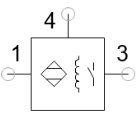
\includegraphics[width=20mm]{../../figures/inductive-sensor.png}};
    \node[yshift=\y cm] at (4,-1.1) {\B};
    \draw[yshift=\y cm] (3.97, 0.6) |- (6, 1); 
    \draw[yshift=\y cm] (-2.0, -0.2) -- ++(5.15, 0); 
    \draw[yshift=\y cm] (4.86, -0.2) --(8, -0.2); 
    
  }
\end{tikzpicture}
\end{document}
